\documentclass[12pt]{article}

\usepackage{sbc-template}
\usepackage{float} 
\usepackage{graphicx,url}
\usepackage[table,xcdraw]{xcolor}

\usepackage[brazil]{babel}   

\usepackage[utf8]{inputenc}  
\pagenumbering{arabic}
     
\sloppy

%ARRUMAR O TITULO
\title{TôAqui: Um aplicativo de chamada automática}

\author{João R. R. de Oliveira\inst{1}, 
Maria Luísa Ghizoni Gonzalez\inst{2}}


\address{Universidade Estadual do Centro-Oeste (UNICENTRO) -- Guarapuava, PR -- Brazil\inst{1}\\
  Departamento de Engenharia Eletrica – Universidade Federal de Minas Gerais (UFMG)\inst{2}
  \email{joaoricardoroliveira@gmail.com,marialuisaghizoni@gmail.com}}
  
  
  
\begin{document}

\maketitle

\begin{abstract}

\end{abstract}



\begin{resumo}

\end{resumo}

\section{Introdução}





\section{Fundamentação Teórica}
Nesta seção é realizada a revisão teórica de textos, artigos, que motivaram o desenvolvimento do projeto. Abaixo é apresentado descrições de trabalhos e aplicativos que envolveram o tema de Frequência em sala de aula automatizado envolvendo \textit{Quick Response Code} (QRCode), Códigos de barra e \textit{Radio-Frequency IDentification} (RFID).


\subsection{Frequencia em sala de aula com \textit{Quick Response Code} (QRCode) e Codigo de barras.}
Com o avanço do uso dos \textit{smartphone} sistemas para registrar e visualizar informações de atendimento usando um código QR escaneado por \textit{smartphones} propôs-se a ajudar os alunos a evitar penalidades que podem resultar de baixa frequência em salas de aula. No sistema proposto, os alunos podem visualizar facilmente os registros de frequência de cada curso. O sistema proposto foi modelado e desenvolvido para uso na Universidade de \textit{Sulaimaniyahm}. No entanto, poderia ser aplicado a outras escolas e faculdades.\cite{QRcode}

Os \textit{smartphones} são mais populares entre os usuários na idade de cerca de 26 anos, usando \textit{smartphones} para acelerar o processo de atendimento por instrutores universitários pouparia tempo de palestras e, portanto, melhorar o processo educacional.\cite{QRcode2}

A frequência escolar determina o desempenho acadêmico de um aluno. O sistema de atendimento estudantil (SAS) que se desenvolveu para o ensino médio em uma escola na malásia, deve substituir o processo de registro de frequência manual. O SAS pode reduzir o tempo gasto pelo professor no cálculo do percentual de frequência para um aluno, bem como para uma turma. Em um clique ou toque de um botão, o professor pode gerar um relatório a qualquer momento. Além disso, a imagem do aluno exibida após o processo de digitalização deve ajudar o professor a identificar os alunos antes de registrar a participação deles.\cite{BarCode}



\subsection{Frequência em sala de aula com RFID}
Com o passar dos anos, as frequências em salas de aulas vem se tornando uma tarefa cansativa para os professores, o que torna possível errar, esquecer de realizar a presença do aluno em sala de aula até mesmo perder os registros de presença \cite{Africa}.

Com o avanço da tecnologia, esse processo pôde ser automatizado utilizando a tecnologia RFID juntamente com um sistema gerenciador web ou mobile.\cite{Africa}
Este sistema pode ser usado em escola, faculdade e universidade. Também pode ser usado prestar assistência aos trabalhadores nos locais de trabalho. Sua capacidade para identificar exclusivamente cada pessoa com base em sua tag RFID. É um tipo de cartão de identificação o qual torna mais fácil, mais rápido e seguro em comparação com outros métodos.\cite{RFIDFrequencia}

O acesso em múltiplo tempo foi um grande problema, no qual, vários cartões tentavam fazer a leitura ao mesmo tempo, o que resultava em cartões que não realizavam a presença.\cite{Africa}


As frequências em salas de aulas são registradas manualmente pelo professor e, portanto, são sujeito a erros pessoais. Com isso, surge a necessidade de criar um método mais eficiente e eficaz de resolver este problema\cite{RFIDemSala}. Uma tecnologia a qual pode resolver este problema e até mesmo fazer muito mais é a tecnologia do RFID\cite{RFIDemSala}.
O RFID é uma tecnologia de identificação e coleta de dados automatizada, que garante uma entrada de dados mais precisa e pontual. 

RFID é uma tecnologia automática e ajuda máquinas ou computadores para identificar objetos, registrar metadados ou controlar alvos individuais através de ondas de rádio. Conectando o leitor de RFID ao terminal de Internet, os leitores podem identificar, rastrear e monitorar os objetos anexados com tags globalmente, automaticamente e em tempo real, se necessário. Esta é a chamada Internet das Coisas (IOT).\cite{RFID2}






\section{Materiais e Métodos}
Nas seções abaixo é detalhada a metodologia e materiais utilizados no desenvolvimento da aplicação.
Esta seção e designada a auxiliar na continuidade do trabalho caso alguém queira reproduzir o mesmo. A seção e dividida em subseções que explicam cada um dos materiais e métodos utilizados.

\begin{itemize}
    \item Bottom-up
        O projeto é iniciado a partir de uma descrição detalhada dos componentes que iram compor o sistema. Esses componentes são conectados para formarem subsistemas, que por sua vez são conectados para formarem subsistemas maiores e assim, sucessivamente até compor o sistema completo.
    
    \item Top-down
    o projeto é iniciado com a formulação geral das características finais do sistema desejado, feita de maneira abstrata, sem detalhes de como será implementado.
    
    \item Meet-in-the-middle
    Essa metodologia é uma combinação das metodologias bottom-up e top-down, buscando aproveitar as vantagens delas e ao mesmo tempo evitando seus problemas. Essa metodologia emprega a abordagem top-down nos níveis de abstração mais altos e a bottom-up nos níveis mais baixos.
    
\end{itemize}

A figura abaixo representa fluxo de projetos embarcados o qual a metodologia Meet-in-the-middle é utilizado. No projeto foi utilizado a metodologia do Meet-in-the-middle e ela será explicada mais abaixo no tópico 4.1.

\begin{figure}[H]
\centering
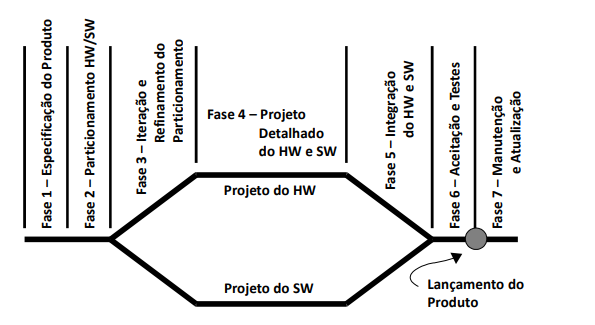
\includegraphics[scale=.6]{FPE.PNG}
\caption{Fluxo de }
\end{figure}




A primeira atividade foi o estudo aprofundado da plataforma do MIT App Inventor, Firebase banco de dados, placas.


Na sequência a segunda atividade foi projetar um aplicativo utilizando a plataforma MIT App Inventor que o aluno fosse capaz de visualizar suas faltas através do smartphone e seus professores pudessem realizar a chamada e conferir a presença dos alunos poupando tempo em sala de aula.

A terceira atividade foi adquirido os materiais necessários para realizar a montagem do protótipo. Após sua montagem foi iniciado testes nas placas o que foi uma etapa muito importante para o protótipo. 
Na quarta atividade, uma vez que as peças não constataram defeitos em seus funcionamentos, foi iniciado a montagem dos componentes no caso o RFID com NodeMCU esp8266.

Em sequencia a quinta atividade foi desenvolver um algoritmo o qual fosse capaz de fazer as duas placas funcionarem em conjunto, que enviassem dados para o aplicativo.

%A sexta atividade foi fazer a conexão do aplicativo e o NodeMcu esp8266 com o servidor MQTT  ??????????????????????


%
%
%  O QUE EU ESCREVO SE NÃO ESTA DANDO CERTO???
%

\subsection{Desenvolvimento da parte Física do Sistema Embarcado}

\subsubsection{Identificação por Radiofrequência (RFID)}
RFID é um acrônimo para "Identificação por radiofrequência" e refere-se a uma tecnologia em que o dados digitais codificados em etiquetas RFID ou etiquetas inteligentes que são capturados por um leitor via ondas de radio. O RFID é semelhante ao código de barras em que os dados de uma \textit{tag} ou rótulo são capturados por um dispositivo que armazena os dados em um banco de dados. 

RFID, no entanto, tem varias vantagens sobre os sistemas que utilizam software de rastreamento. O mais notável é que os dados das etiquetas RFID podem ser lidos fora da linha de visão enquanto os códigos de barras devem estar alinhados com um \textit{scanner} ótico.

Em um nível simples, os sistemas RFID consistem em três componentes: uma etiqueta RFID ou etiqueta inteligente, um leitor RFID e uma antena. As etiquetas RFID contêm um circuito integrado e uma antena, que são usados para transmitir dados ao leitor RFID (também chamado de interrogador). O leitor então converte as ondas de rádio em uma forma mais utilizável de dados. As informações coletadas das \textit{tags} são então transferidas através de uma interface de comunicação para um sistema de computador \textit{host}, onde os dados podem ser armazenados em um banco de dados e analisados posteriormente.

Uma etiqueta RFID consiste em um circuito integrado e uma antena. A etiqueta também é composta de um material protetor que mantém as peças juntas e protege-as de várias condições ambientais. O material de proteção depende da aplicação. Por exemplo, os crachás de identificação de funcionários que contêm etiquetas RFID são normalmente feitos de plástico durável e a \textit{tag} é incorporada entre as camadas de plástico. As etiquetas RFID vêm em uma variedade de formas e tamanhos e são passivas ou ativas. As \textit{tags} passivas são as mais usadas, pois são menores e menos dispendiosas de implementar. As \textit{tags} passivas devem ser "ativadas" pelo leitor de RFID antes que elas possam transmitir dados. Ao contrário das \textit{tags} passivas, as etiquetas RFID ativas têm uma fonte de alimentação integrada (por exemplo, uma bateria), permitindo que elas transmitam dados o tempo todo.



\subsubsection{NodeMCU esp8266}


O NodeMCU exp8266 é uma placa wifi de desenvolvimento que combina o chip ESP8266, uma interface usb-serial e um regulador de tensão 3.3V. A programação pode ser feita usando LUA ou a IDE do Arduino, utilizando a comunicação via cabo micro-usb. 
A placa possui uma memória de física de 4 MegaBytes e opera em um frequência 80MHz / 160MHz.

É uma placa amplamente utilizada para desenvolvimento IoT, pois contém conexão com a internet podendo ser acessada de qualquer lugar do mundo após a sua programação.

\begin{figure}[H]
\centering
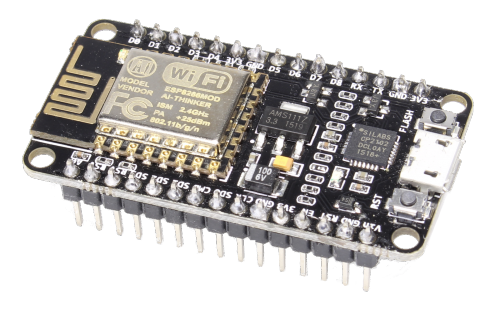
\includegraphics[scale=.3]{node.png}
\caption{Placa WIFI NodeMCU esp 8266.}
\end{figure}


\subsection{Desenvolvimento do Software embarcado}

%\subsubsection{\textit{Message Queuing Telemetry Transport} (MQTT)}

%O protocolo MQTT é a sigla para \textit{Message Queuing Telemetry Transport}, ou seja, é o protocolo de mensagens entre máquinas. Desenvolvido pela IBM no final dos anos 90, ele tinha como objetivo principal ajudar na comunicação entre sensores e satélites. Hoje, o MQTT é utilizado de diversas formas, especialmente em IoT e nas automações residenciais. Também é ideal para aplicativos móveis devido ao seu tamanho pequeno, baixo consumo de energia, pacotes de dados minimizados e distribuição eficiente de informações para um ou vários receptores.


 %De forma bem geral e resumida, o processo é basicamente:

%\begin{itemize}
 %   \item Uma mensagem é enviada ao broker, que é capaz de compreender e ler múltiplos aparelhos ao mesmo tempo;
  %  \item Através da base de TCP/IP, é realizado a leitura das mensagens;
   % \item Os sensores de diversos aparelhos então podem se comunicar e trabalhar juntos.
%\end{itemize}

%O Broker é como uma espécie de mediador entre as máquinas, capaz de fazer com que a comunicação de fato ocorra entre elas. 




\subsubsection{MIT App Inventor}

O MIT App Inventor é um ambiente de programação intuitivo o que permite que até crianças criem aplicativos funcionais para smartphone ou tablet. 
Pode-se ter um aplicativo funcional em menos de 30 minutos através da plataforma do MIT. A ferramenta de programação é baseada em blocos o que facilita a criação de aplicativos mais complexos e diminui altamente o tempo de ambientes de programações tradicionais.
A Ferramenta oferece dois ambientes de trabalho o ambiente \textit{Design} e o ambiente \textit{Blocks}.
O ambiente \textit{Design} é composto por vários componentes de layout, interface do usuário, mídia, desenho e animação, mapa, sensor, sociais, armazenamento, conectividade e componentes experimentais.

Os blocos são separados por blocos de controle, lógicos, matemáticos, texto, cores, variáveis, procedimentos, listas. Dentro desses blocos existem vários sub-blocos que contém um função mais especifica. 


\subsubsection{Google Firebase}

O \textit{Google Firebase} é uma plataforma de desenvolvimento mobile/web o qual a empresa \textit{Google} é responsável.
É um serviço em nuvem para desenvolvedores com foco principal de ser um \textit{back-end} completo e de muita facilidade de ser utilizado, disponibilizando diversos serviços diferentes que auxiliam no gerenciamento e desenvolvimento de aplicativos.

O serviço de \textit{Realtime Database} que é um banco de dados que sincroniza os dados com os dispositivos em tempo real, podendo configurar regras de segurança e definir quem tem acesso a determinado arquivo do banco de dados.

O \textit{Firebase} oferece serviços muito bom e de fácil implementação, e a maioria dos serviços oferecidos pode ser utilizada de forma gratuita para pequenos projetos.

A segurança de que os dados serão bem armazenados e que sempre estarão em segurança é uma das principais funções do banco. A criptografia que contém é suficiente para a segurança, o espaço de armazenamento para a realização do protótipo, funções próprias e únicas que possam auxiliar, ações automáticas que previnem perda de dados entre outros

\subsubsection{IDE Arduino}
Arduíno \textit{Integrated Development Environment}(IDE) é um Ambiente de Desenvolvimento Integrado que é ferramente muito utilizada para desenvolvimento de produtos IoT. Pode ser utilizado para o desenvolvimento de projetos interativos independentes ou conectado a um computador. Contém uma interface de programação bem simples de ser utilizada.

\begin{figure}[H]
\centering
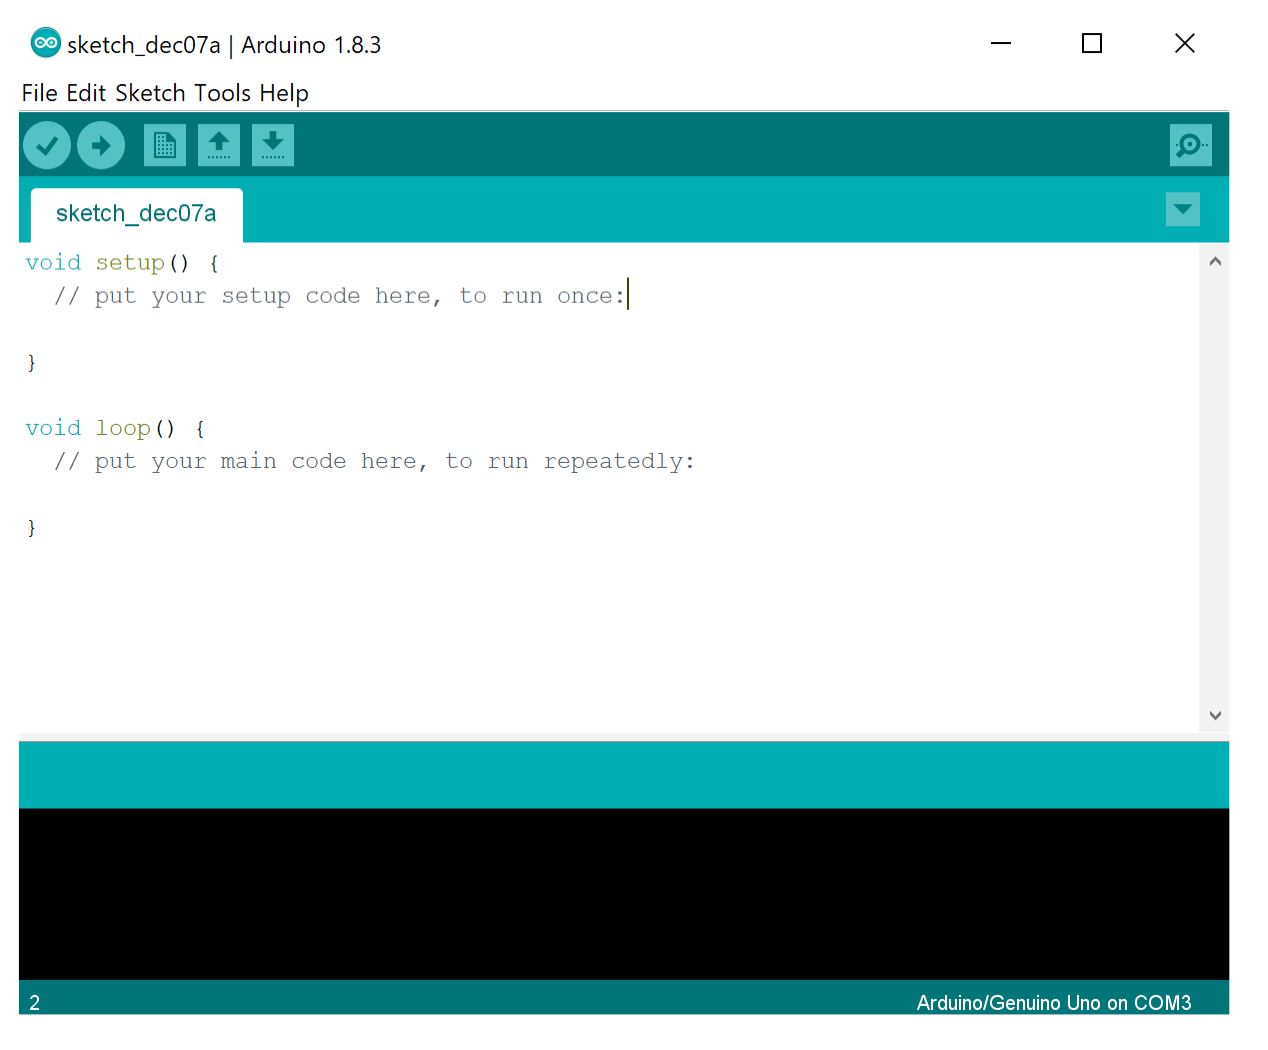
\includegraphics[scale=.30]{arduinoide.png}
\caption{IDE Arduíno quando aberta a primeira vez.}
\end{figure}


\section{Desenvolvimento}
Nesta seção é descrito o desenvolvimento do aplicativo, o desenvolvimento do projeto embarcado, a comunicação com o banco de dados e a comunicação com o servidor.

\subsection{Especificação do produto}
A ideia principal do projeto é um sistema de controle de presenças automatizado o qual o aluno sempre que for ingressar em uma sala de aula, vai passar seu RA(Registro Acadêmico), o qual estará equipado com a etiqueta RFID internamente, o que irá registrar a presença automaticamente. Podendo também o aluno em um aplicativo em seu smartphone, ter o controle de suas faltas.

O diagrama de classe de uso abaixo mostra como o sistema é projetado e como deve funcionar. Porém o aplicativo ainda não conta com um sistema de login e subdivisões no banco de dados Firebase. 

\begin{figure}[H]
\centering
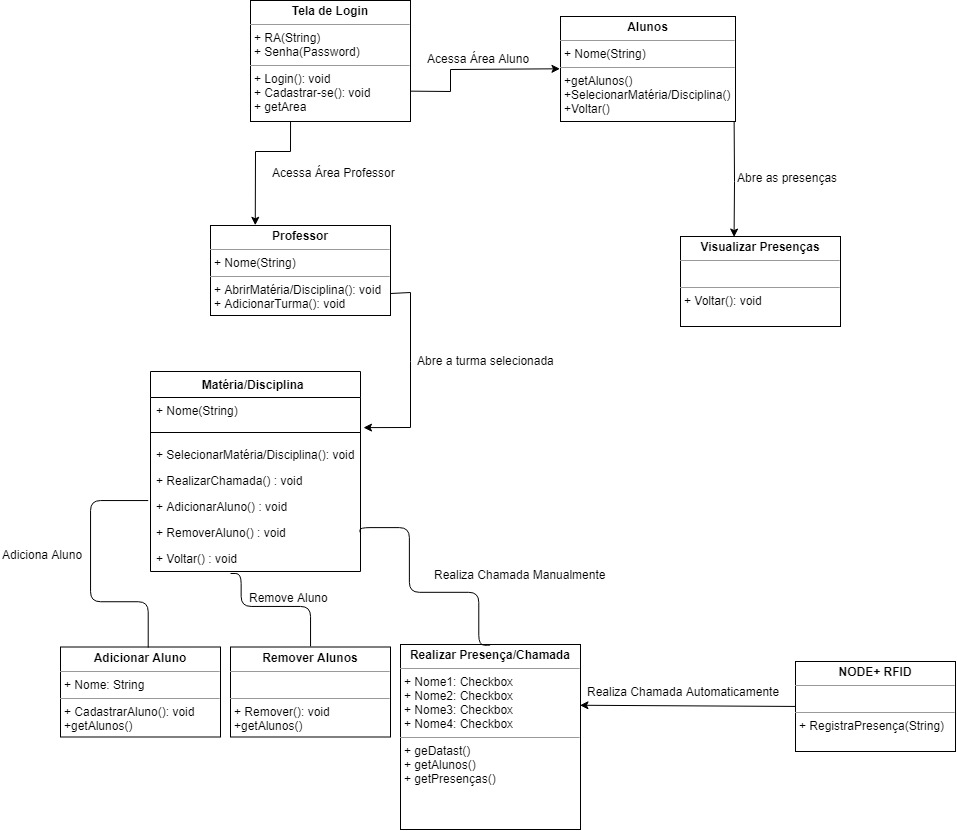
\includegraphics[scale=.35]{DCU.jpg}
\caption{Diagrama de classe do aplicativo TôAqui.}
\end{figure}


\subsection{Particionamento do projeto em componentes de hardware e software}

O projeto foi sub dividido em duas partes, hardware e software. O desenvolvido da parte do software teve inicio antes da parte do hardware por questões de requisitos e prioridades. No entanto essa decisão deve ser notada propriamente na fase 4.1

O desenvolvimento do software teve inicio com a idealização de um modelo composto com as frequências em salas sendo preenchidas em check-box com datas e alunos já cadastrados no banco de dados, facilitando e poupando tempo para o início do projeto.

Então após a realização desta etapa principal no aplicativo foi divido ele em duas partes, área "Aluno" e área "Professor" o qual o aluno somente pode visualizar suas frequências nas aula, e o professor podendo realizar a chamada, adicionar e remover o aluno da sua lista de presença, o que muitas vezes é preciso em caso o aluno desista ou ingresse futuramente um novo aluno em sua turma.

Com o desenvolvimento pronto das duas áreas a próxima etapa foi a conexão com o banco de dados firebase o qual foi bastante simples, pois não necessita instalar nenhum software ou \textit{driver} especifico como muitos bancos de dados requerem.

\begin{figure}[H]
\centering
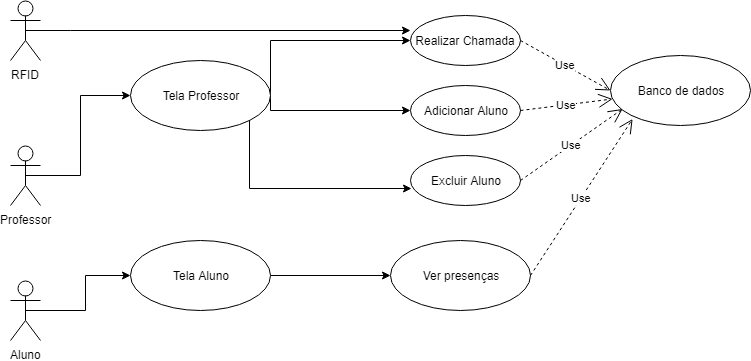
\includegraphics[scale=.50]{TCC-APP.png}
\caption{Diagrama de caso de uso do Aplicativo TôAqui.}
\end{figure}

\subsection{Iteração e refinamento do particionamento}
Nesta etapa foram realizados diversos testes nos componentes e nas plataformas que foram utilizadas. Nenhum dos componentes eletrônicos falhou em algum momento, sendo aptos para realizar o trabalho requisitado.

Já as plataformas utilizadas apenas a plataforma do MIT apresentou pequenos travamentos ou até mesmo fechamentos durante a realização. As demais plataformas utilizadas obtiveram exito em suas funcionalidades.

\subsection{Tarefas independentes de projeto do hardware e do software}
O projeto de \textit{hardware} o qual a função principal do NodeMCU esp8266 é fazer dele um servidor o qual irá realizar a comunicação do RFID com o aplicativo.
A placa MRFC522 que registra a leitura da etiqueta RFID sua função é capturar o código do cartão, transformar em hexadecimais e repassar para o NodeMCU repassar as informações.

A figura representada abaixo mostra como foi realizada a conexão através de fios(Jumpers) do NodeMcu com o RFID.
\begin{figure}[H]
\centering
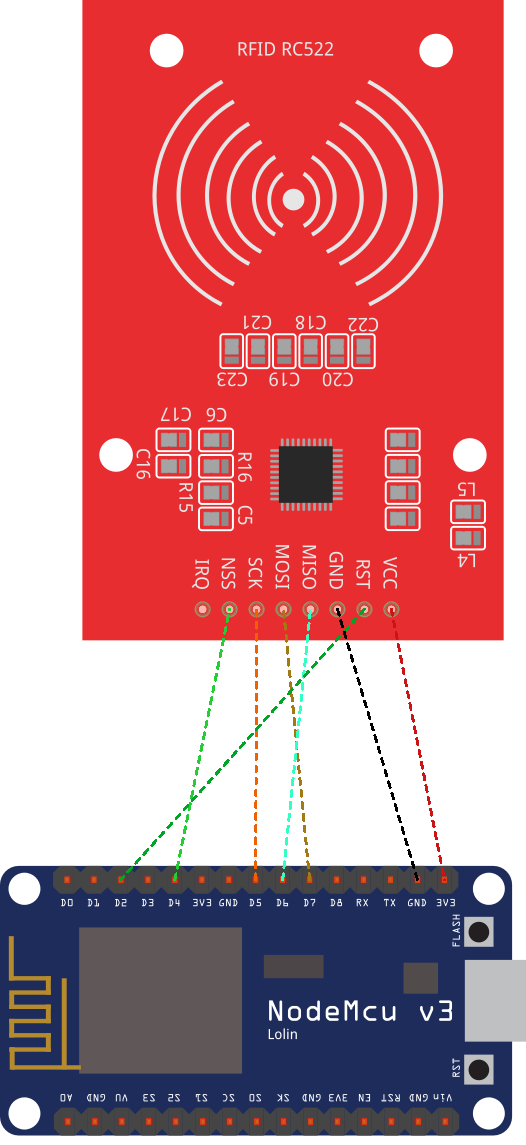
\includegraphics[scale=.70]{SketchArduino.png}
\caption{Modelagem do projeto embarcado.}
\end{figure}

Já no projeto do \textit{software} onde o aplicativo foi desenvolvido na plataforma do MIT o software é responsável por todos os toques e ações que o usuário irá realizar, o software também realiza a conexão com o banco de dados Firebase o qual apenas foi utilizado uma \textit{Application Programming Interface}(API Key), que no português significa Chave de Interface de Programação de Aplicações para realizar a ligação entre o banco de dados e o aplicativo.


%
% COLOCAR FOTO DO APP
%

\subsection{Integração dos componentes de hardware e software}

%
%  FALTA PARTE DO HARDWARE O QUAL THIERRY VAI ME AJUDAR AMANHA
%
A união das duas partes .........
No momento de Integração da parte do hardware com a parte software ocorreu diversos problemas com a parte do \textit{hardware} pois as duas placas não se comunicavam como deveriam e acabavam travando e não realizando as ações requisitadas no projeto.


\subsection{Testes, aceitação e lançamento do produto}
Durante a execução do aplicativo sem a integração dele com os componentes de hardware foram realizados diversos testes induzindo ao erro, contudo o aplicativo não apresentou falhas durante os testes realizados.

%
%  FALTA PARTE DO HARDWARE O QUAL THIERRY VAI ME AJUDAR AMANHA
%

\subsection{Manutenção e atualização contínua}
%
% O QUE ESCREVO AQUI???
%

O aplicativo não tera atualizações futuras, pois foi apenas uma versão para fortalecer a ideia, futuramente podendo a ser implementado em uma linguagem de programação melhor e mais desenvolvida mundialmente.






\section{Resultados e Discussões}

\section{Considerações Finais}

\section{Agradecimentos}


\bibliographystyle{plain}
\bibliography{references}


\end{document}
